
%(BEGIN_QUESTION)
% Copyright 2008, Tony R. Kuphaldt, released under the Creative Commons Attribution License (v 1.0)
% This means you may do almost anything with this work of mine, so long as you give me proper credit

Calculate the current and all voltage drops in this loop-powered transmitter circuit, assuming the pressure transmitter is calibrated for a range of 50 to 150 PSI, 4 to 20 mADC.  Be sure to show all your work!

$$\includegraphics[width=15.5cm]{i03141x01.eps}$$

% No blank lines allowed between lines of an \halign structure!
% I use comments (%) instead, so that TeX doesn't choke.

$$\vbox{\offinterlineskip
\halign{\strut
\vrule \quad\hfil # \ \hfil & 
\vrule \quad\hfil # \ \hfil & 
\vrule \quad\hfil # \ \hfil & 
\vrule \quad\hfil # \ \hfil \vrule \cr
\noalign{\hrule}
%
% First row
Applied & Current & Transmitter & Resistor \cr
%
pressure (PSI) & (mA) & voltage (V) & voltage (V) \cr
%
\noalign{\hrule}
%
% Another row
55 PSI &  &  &  \cr
%
\noalign{\hrule}
%
% Another row
70 PSI &  &  &  \cr
%
\noalign{\hrule}
%
% Another row
82 PSI &  &  &  \cr
%
\noalign{\hrule}
%
% Another row
107 PSI &  &  &  \cr
%
\noalign{\hrule}
%
% Another row
140 PSI &  &  &  \cr
%
\noalign{\hrule}
%
% Another row
150 PSI &  &  &  \cr
%
\noalign{\hrule}
} % End of \halign 
}$$ % End of \vbox

\vfil 

\underbar{file i03141}
\eject
%(END_QUESTION)





%(BEGIN_ANSWER)

This is a graded question -- no answers or hints given!

%(END_ANSWER)





%(BEGIN_NOTES)

% No blank lines allowed between lines of an \halign structure!
% I use comments (%) instead, so that TeX doesn't choke.

$$\vbox{\offinterlineskip
\halign{\strut
\vrule \quad\hfil # \ \hfil & 
\vrule \quad\hfil # \ \hfil & 
\vrule \quad\hfil # \ \hfil & 
\vrule \quad\hfil # \ \hfil \vrule \cr
\noalign{\hrule}
%
% First row
Applied & Current & Transmitter & Resistor \cr
%
pressure (PSI) & (mA) & voltage (V) & voltage (V) \cr
%
\noalign{\hrule}
%
% Another row
55 PSI & 4.8 & 25.8 & 1.2 \cr
%
\noalign{\hrule}
%
% Another row
70 PSI & 7.2 & 25.2 & 1.8 \cr
%
\noalign{\hrule}
%
% Another row
82 PSI & 9.12 & 24.72 & 2.28 \cr
%
\noalign{\hrule}
%
% Another row
107 PSI & 13.12 & 23.72 & 3.28 \cr
%
\noalign{\hrule}
%
% Another row
140 PSI & 18.4 & 22.4 & 4.6 \cr
%
\noalign{\hrule}
%
% Another row
150 PSI & 20.0 & 22.0 & 5.0 \cr
%
\noalign{\hrule}
} % End of \halign 
}$$ % End of \vbox


%INDEX% Electronics review: 4-20 mA loop circuits

%(END_NOTES)


